\chapter{The pn junction}\label{c2}
\section{Semiconductor junctions}\label{c2s1}
Metal-semiconductor junctions were known even before the semiconductor diode
became popular. Crystal rectifiers were used in microwave and radio-frequency
electronics even befoce vacuum tube diodes were developed. These junctions were
between crystals of different materials. In this chapter, we will consider a
junction formed by a sharp transition of impurity concentration in a single
crystal. The junction has its origin in the chemical and not mechanical 
inhomogeneity. We will largely follow the treatment in Shockley's 
\cite{shockley1949theory} paper of 1949.

Figure \ref{fig1} shows the schematic diagram of a pn junction, published in
Shockley's paper \cite{shockley1949theory}
\begin{figure}[htbp]
\centering
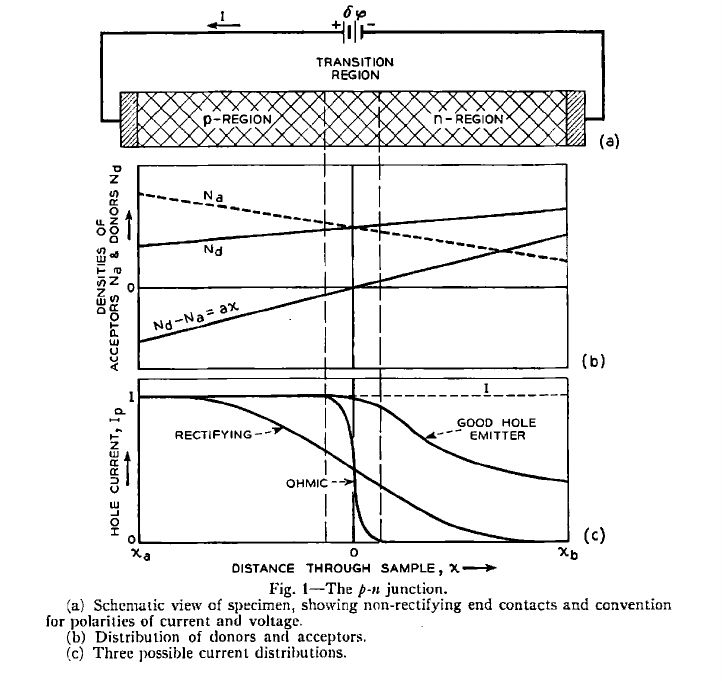
\includegraphics[width=0.95\textwidth]{pn-junction-shockley1949}
\caption{A p-n junction}
\label{fig1}
\end{figure}

The p-side has an excess of acceptor impurity over donor impurity. The situation
is the other way round on the n-side. The junction exists at a point where 
$N_A = N_D$. The concentration $|N_A - N_D|$ is small in a neighbourhood of the
junction, call the \emph{transition layer}. Beyond the transition layer, the
impurity concentration is substantial. 

A rectifying junction is formed when charge carriers diffuse across the 
junction. The electrons diffusing across the junction combine with the holes
resulting in a drop in hole current as we approach the junction. The hole
diffuse across the junction resulting in a decreasing hole current on the
n-side of the junction. Likewise, the electon current starts dropping as we
approach the junction from the n-side and it persists for some distance in the
p-side.

If the junction has many defects or recombination centres then the electrons
diffusing from the n-side are mostly combined with the holes arriving from the
opposite direction in the close vicinty of the junction. There is hardly any
diffusion of minority carriers across the junction. The transition layer is
extremely narrow or non-existent. As a result, when the device is 
reverse-biased, there is a copious generation of electron-hole pairs at the
junction and no drop in current compared to when the device is forward-biased.
Such a junction is a non-rectifying junction.

\section{The transition region}\label{c2s2}
The density of electrons in the conduction band is given by \eqref{c1e3} as
\[
n = N_C e^{-\beta(E_c - \mu)},
\]
where $N_C$ is the density of states, $E_c$ the lowest energy in the conduction
band and $\mu$ is the chemical potential. As long as the doping is not 
excessive, the presence of dopants does not appreciable change the crystal 
structure of the host. As a result, the band structure is unchanged and so is
the density of states. However, the chemical potential shifts because of 
impurities. We observed in equations \eqref{c1e43} (\eqref{c1e44}) that the
presence of donor (acceptor) impurities pushes the chemical potential upwards
(downwards), closer to $E_c$ ($E_v$). In this section, we shall call the 
chemical potential of the intrinsic crystal $\mu_i$. Thus, we have \eqref{c1e13}
for a doped crystal and
\begin{equation}\label{c2e1}
n_i = N_c e^{-\beta(E_c - \mu_i)}
\end{equation}
as its analogue for the pure crystal. Taking their ratio, we get
\begin{equation}\label{c2e2}
\frac{n}{n_i} = e^{-\beta(\mu - \mu_i)}.
\end{equation}
Similarly, for the hole concentration, we have
\begin{equation}\label{c2e3}
\frac{p}{p_i} = e^{-\beta(\mu_i - \mu)}.
\end{equation}
When the crystal is placed in an electric potential $V(x)$, its internal, 
periodic potential shifts by that amount. All energy levels shift. However, 
the differences between them, like the band gap, remain unchanged. We now
choose the zero of our potential at $\mu_i$ so that when we apply the voltage,
the chemical potential of the intrinsic crystal becomes $\mu_i = -eV$, $e > 0$ 
being the elementary charge. If we also write $\mu = -e\varphi$ then equations
\eqref{c2e2} and \eqref{c2e3} become
\begin{eqnarray}
n &=& n_i e^{\beta e(V - \varphi)} \label{c2e4} \\
p &=& n_i e^{\beta e(\varphi - V)} \label{c2e5}
\end{eqnarray}
where we used the fact that $p_i = n_i$ for an intrinsic semiconductor. If
$N_D$ and $N_A$ are the concentrations of donor and acceptors then the total
charge density is
\begin{equation}\label{c2e6}
\rho = e(p - n + N_D - N_A),
\end{equation}
which, using \eqref{c2e4} and \eqref{c2e5} becomes
\begin{equation}\label{c2e7}
\rho = e(N_D - N_A + 2n_i\sinh(\beta e (\varphi - V)).
\end{equation}

There is a further modification to the chemical potential when there is an
injection of carriers or their generation due to other means like light. If
we denote it be $\varphi_n$ and $\varphi_p$ for the electrons and holes
respectively, we get
\begin{eqnarray}
n &=& n_i e^{\beta e(V - \varphi_n)} \label{c2e8} \\
p &=& n_i e^{\beta e(\varphi_p - V)}. \label{c2e9}
\end{eqnarray}
The net hole current is due to diffusion as well as drift. Thus,
\begin{equation}\label{c2e10}
\vec{J}_q = -eD_p\grad{p} - e\mu_p p \grad{V},
\end{equation}
where $D_p$ is the hole diffusion constant and $\mu_p$ is the hole mobility.
From equation \eqref{c2e9},
\[
\grad p = pe\beta(\grad\varphi_p - \grad V)
\]
so that \eqref{c2e10} becomes
\[
\vec{J}_p = -pe^2\beta D_p\grad\varphi_p + pe^2\beta D_p\grad V - 
e\mu_p p\grad{V}.
\]
Using equation \eqref{c1e46}, the last two terms cancel each other and we get
\begin{equation}\label{c2e11}
\vec{J}_p = -e\mu_p p \grad\varphi_p.
\end{equation}
Likewise, we have
\begin{equation}\label{c2e12}
\vec{J}_n = -e\mu_n n \grad\varphi_n = -eb\mu_p n\grad\varphi_n,
\end{equation}
where $b = \mu_n/\mu_p$ is the ratio of the mobility of the two carriers.

